\loai{Loại 1. Nhận nhiệt, nhận công}
\begin{ex}
	Một lượng khí nhận nhiệt lượng $250 \ kJ$ do được đun nóng; đồng thời nhận công $500 \ kJ$ do bị nén. Độ tăng nội năng của lượng khí bằng 
	\choice
	{500 kJ}
	{250 kJ}
	{\True 750 kJ}
	{700 kJ}
	\loigiai{
		\begin{itemize}
			\item Độ tăng nội năng $\Delta U=Q+A=250+500=750\ kJ$
		\end{itemize}
	}
	\haidong{4}\end{ex}






\loai{Loại 2. Nhận nhiệt, sinh công}
\begin{ex}
	\immini[thm]{Một lượng khí nóng được chứa trong một xi-lanh đặt nằm ngang, pit-tông có thể di chuyển được. Không khí nóng dãn nở đẩy pit-tông dịch chuyển. Khối khí nóng bên trong xi-lanh thực hiện một công có độ lớn là $4000\ J$. Bỏ qua sự trao đổi nhiệt của xi-lanh với môi trường.}{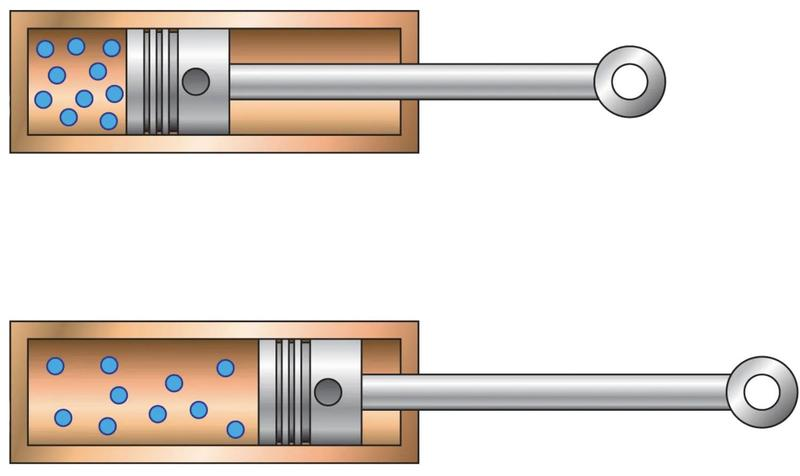
\includegraphics[width=4cm]{Images/xilanh1}}
	
	\begin{chc}
		Nội năng của khối khí biến thiên một lượng bằng
		\choice
		{$4000\ J$}
		{$-8000\ J$}
		{\True $-4000\ J$}
		{$0\ J$}
		\loigiai{
			\begin{itemize}
				\item[A] Sai. Dấu sai, vì khí thực hiện công nên nội năng giảm.
				\item[B] Sai. Nhầm hệ số, không có lý do nhân đôi.
				\item[C] Đúng. $Q = 0 \Rightarrow \Delta U = Q + A = 0 - 4000 = -4000\ J$
				\item[D] Sai. Nội năng giảm do khí thực hiện công.
			\end{itemize}
		}
	\end{chc}
	
	\begin{chc}
		Sau đó, khí nhận thêm nhiệt lượng $10000\ J$ và thực hiện thêm $1500\ J$ công. Nội năng biến thiên một lượng bao nhiêu kể từ khi nó bắt đầu dãn nở?
		\choice
		{$2500\ J$}
		{\True $4500\ J$}
		{$5500\ J$}
		{$-1500\ J$}
		\loigiai{
			\begin{itemize}
				\item[A] Sai. Đây là hiệu $10000 - 7500$ (nếu nhầm công tổng là 7500\ J).
				\item[B] Đúng. $\Delta U = Q + A = 10000 - 5500 = 4500\ J$
				\item[C] Sai. 5500\ J là tổng công chứ không phải nội năng.
				\item[D] Sai. Nội năng không giảm, vì $Q > A$.
			\end{itemize}
		}
	\end{chc}
\end{ex}



\begin{ex}%[1P6-3.2B][Loai1] 
	Người ta truyền cho khối khí trong xi-lanh nhiệt lượng 100 J. Khí nở ra thực hiện công 80 J, đẩy pit-tông lên. Độ biến thiên nội năng của khối khí là
	\choice
	{\True 20 J}
	{40 J}
	{180 J}
	{120 J}
	\loigiai{\begin{itemize}
			\item Khí nhận nhiệt: $Q=100\ J$.
			\item Khí dãn nở sinh công: $A=-80\ J$.
			\item Độ biến thiên nội năng của khí: $\Delta U=A+Q=20\ J$.
	\end{itemize}}
	\haidong{3}\end{ex}



\begin{ex} \nguon{1}
	Một khối khí được truyền một nhiệt lượng $2000 \ J$ thì khối khí dãn nở và thực hiện được một công $1500 \ J$. Độ biến thiên nội năng của khối khí là
	\choice
	{\True $500 \ J$}
	{$3500 \ J$}
	{$-3500 \ J$}
	{$-500 \ J$}
	\loigiai{
		\begin{itemize}
			\item 
			$\Delta U = Q + A = 2000  - 1500  = 500 \ J$
\end{itemize}
	}
\end{ex}


\begin{ex} \nguon{4}
	Người ta cung cấp cho một khối khí trong xi-lanh nhiệt lượng $50 \ J$, chất khí nở ra và đẩy pit-tông lên thực hiện một công là $30 \ J$. Độ biến thiên nội năng của khối khí là bao nhiêu jun
	\shortans[oly]{ 20}
	\loigiai{
		\begin{itemize}
			\item Khí nhận nhiệt lượng và thực hiện công nên: $Q>0$ và $A<0$
			\item Độ biến thiên nội năng: $\Delta U=Q+A=50-30=20 \ J$
			\item Vậy nội năng của khối khí tăng thêm $20 \ J$.
		\end{itemize}
	}
\end{ex}


\loai{Loại 3. Nhận công, tỏa nhiệt}
\begin{ex}%[1P6B3-2][Loai1] 
	Người ta thực hiện công 200 J để nén khí trong một xi-lanh. Khí truyền ra môi trường xung quanh nhiệt lượng 40 J. Độ biến thiên nội năng của khí là
	\choice
	{\True 160 J}
	{100 J}
	{200 J}
	{400 J}
	\loigiai{
		\begin{itemize}
			\item Khí tỏa nhiệt: $Q=-40\ J$.
			\item Khí nhận công: $A=200\ J$.
			\item Độ biến thiên nội năng của khí: $\Delta U=A+Q=200-40=160J $.
	\end{itemize}}
	%<MyLT>
	\haidong{6}\end{ex}




\begin{ex}
	Người ta thực hiện công 1000 J để nén khí trong xi-lanh, khí truyền ra bên ngoài nhiệt lượng \(600 \ \text{J}\). Độ biến thiên nội năng của khí là
	\choice
	{$1000 \ \text{J}$}
	{$600 \ \text{J}$}
	{$300 \ \text{J}$}
	{\True $400 \ \text{J}$}
	\loigiai{
		Theo định luật I của nhiệt động lực học, độ biến thiên nội năng \(\Delta U\) được tính bằng:
		\[ \Delta U = A + Q \]
		Ở đây, \(A = 1000 \ \text{J}\) là công hệ nhận được (dương), \(Q = -600 \ \text{J}\) là nhiệt lượng truyền ra khỏi hệ (âm).
		Do đó:
		\[ \Delta U = 1000 \ \text{J} + (-600 \ \text{J}) = 400 \ \text{J} \]
		Vậy độ biến thiên nội năng của khí là \(400 \ \text{J}\).
	}
	\haidong{5}
\end{ex}


\begin{ex}
	Người ta thực hiện công $1000 \ J$ để nén khí trong một xi-lanh. Biết khí truyền ra môi trường xung quanh nhiệt lượng $400 \ J$. Độ biến thiên nội năng của khối khí là
	\choice
	{$1400 \ J$}
	{\True $600 \ J$}
	{$-600 \ J$}
	{0}
	\loigiai{
		Độ biến thiên nội năng: $\Delta U=A+Q=1000-400=600\ J$.
	}
	\haidong{5}\end{ex}
	
\begin{ex} \nguon{4}
	Người ta thực hiện một công $120 \ J$ để nén một khối khí trong xi-lanh, khi đó khối khí truyền ra bên ngoài một nhiệt lượng $40 \ J$. Độ biến thiên nội năng của khối khí là bao nhiêu jun?
	\shortans[oly]{80} 
	\loigiai{
		\begin{itemize}
			\item Khí nhận công và truyền nhiệt nên: $A>0$ và $Q<0$
			\item Độ biến thiên nội năng của khối khí: $\Delta U=Q+A=-40+120=80 \ J$
			\item Vậy nội năng của khối khí tăng thêm $80 \ J$.
		\end{itemize}
	}
\end{ex}
\loai{Loại 4. Tính công}

\loai{Loại 5. Tính nhiệt lượng}

\begin{ex}%[1P6B3-2][Loai2] 
	Người ta thực hiện công 40 J lên khối khí trong xi-lanh làm cho nội năng khối khí tăng thêm 20 J thì khối khí
	\choice
	{\True tỏa nhiệt 20 J}
	{nhận nhiệt 20 J}
	{tỏa nhiệt 40 J}
	{nhận nhiệt 40 J}
	\loigiai{
		\begin{itemize}
			\item Thực hiện công lên khối khí suy ra khí nhận công: $A=40\ J$.
			\item Nội năng của khí tăng: $\Delta U=20\ J$.
			\item Nhiệt lượng khí nhận được: $Q=\Delta U-A=-20\ J\Rightarrow$ khối khí tỏa nhiệt 20 J.
	\end{itemize}}
	%<MyLT2>
	\haidong{5}\end{ex}




\loai{Loại 6. Tính công do khí thực hiện rồi tính độ biến thiên nội năng}
\begin{ex}
	\immini[thm]{Người ta cung cấp nhiệt lượng $1,5\ J$ cho chất khí đựng trong một xi-lanh đặt nằm ngang. Chất khí nở ra, đẩy pit-tông chuyển động thẳng đều và đi một đoạn $5 \ cm$. Biết tổng lực cản của khí ngoài xi-lanh và lực ma sát giữa pit-tông và xi-lanh có độ lớn không đổi là $20\ N$. Độ biến thiên nội năng của chất khí là
		%	}{\begin{tikzpicture}[scale=1,thick,>=stealth']
			%		\tkzDefPoints{0/0/o, -2.15/-0.1/a, -1.25/-0.1/b}
			%		\draw (0,0) -- (-3.5,0) -- (-3.5,1) -- (0,1);
			%		\draw (-0.75,1) -- (-0.75,0);
			%		\draw (-1.25,1) -- (-1.25,0);
			%		\fill[pattern=north east lines] (-1.25,0)rectangle(-0.75,1);
			%		\draw[dashed] (-1.75,1) -- (-1.75,0);
			%		\draw[dashed] (-2.15,1) -- (-2.15,0);
			%		\draw [decorate,decoration={brace,mirror,amplitude=5pt},xshift=0pt,yshift=-4pt]
			%		(a) -- (b) node [black,midway,yshift=-15pt] 
			%		{\footnotesize $\Delta \ell$};
			%		\end{tikzpicture}}
	\choice
	{$4,0\ J$}
	{$2,0\ J$}
	{\True 0,5 J}
	{$2,5\ J$}}{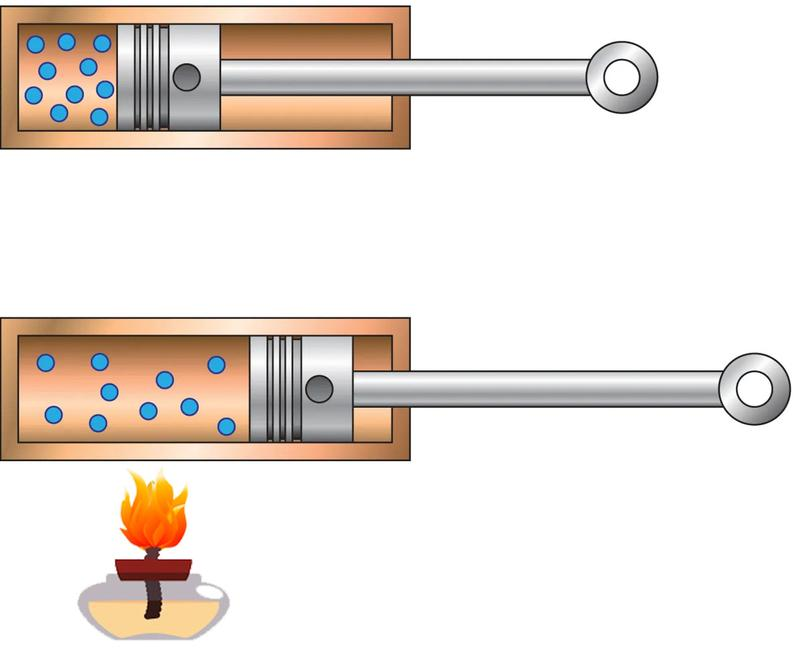
\includegraphics[width=4cm]{Images/xilanh2}}
\loigiai{
	\begin{itemize}
		\item Do pít-tông chuyển động đều nên lực do khí tác dụng lên pít-tông bằng với lực cản nên $F=F_c$
		\item Công mà khí thực hiện có độ lớn là: $|A|=|F|. s=20.0,05=1\ J$.
		\item Khí thực hiện công nên $A=-1\ J$		
		\item Độ biến thiên nội năng của khối khí: $\Delta U=Q+A=1,5-1=0,5\ J$.
	\end{itemize}
	
	%		\begin{center}
		%			
\includegraphics[width=4cm]{images/2024_04_20_47fa5b18dc83027611bdg-05(2)}
		%		\end{center}
	
}
\haidong{11}\end{ex}



\begin{ex}
Một khối khí chứa trong một xi-lanh đặt thẳng đứng có pit-tông trọng lượng không đáng kể, diện tích đáy $10 \ cm^2$, có thể dịch chuyển được. Biết nhiệt độ của khí không đổi, áp suất khí quyển bằng $101325\ Pa$, và công khí sinh ra trong quá trình này là $7,5\ J$. Công cần thực hiện để kéo pit-tông lên cao thêm $10 \ cm$ là
\choice
{$2,31\ J$}
{\True $2,63\ J$}
{$17,63\ J$}
{$7,5\ J$}
\loigiai{	
\begin{itemize}
	\item Gọi áp suất do khối khí tác dụng lên pit-tông là $p_1=\dfrac{F_1}{S}=\dfrac{A_1}{Sh}$;\\ 
	\item Áp suất do lực kéo tác dụng lên pit-tông là $p_2=\dfrac{F_2}{S}=\dfrac{A_2}{Sh}$;\\
	\item Áp suất do khí quyển tác dụng lên pit-tông là $p_3=101325\ Pa$.
	\item Khi pít-tông cân bằng thì áp suất phía trong và phía ngoài pit-tông cân bằng nhau. 
	\begin{align*}
		p_1+p_2=p_3\Rightarrow \dfrac{A_1+A_2}{Sh}=p_3\Rightarrow A_2=p_3.Sh-A_1=101325.10.10^{-4}.0,1-7,5=2,6325\ J
	\end{align*}
	\end{itemize}}
	
	\haidong{8}\end{ex}


\begin{ex}
Người ta cung cấp nhiệt lượng $25 \ J$ cho một lượng khí trong xi-lanh đặt nằm ngang. Lượng khí nở ra đẩy pit-tông chuyển động thẳng đều trong xi-lanh được $10 \ cm$. Bỏ qua áp suất không khí bên ngoài xi-lanh. Biết tổng lực cản tác dụng lên pit-tông có độ lớn $20 \ N$. Độ biến thiên nội năng của lượng khí là
\choice
{$20 \ J$}
{$27 \ J$}
{\True $23 \ J$}
{$25 \ J$}
\loigiai{
\begin{itemize} 
	\item Do pít-tông chuyển động đều nên lực do khí tác dụng lên pít-tông bằng với lực cản nên $F=F_{ms}$
	\item Công mà khí thực hiện có độ lớn là: $|A|=F.d=20.0,1=2\ J$.
	\item Khí thực hiện công nên $A=-2\ J$
	\item Độ biến thiên nội năng của khối khí: $\Delta U=Q+A=Q-A'=25-2=23\ J$. 
	\item Nội năng của chất khí tăng thêm 23 J.
\end{itemize}
}
\haidong{8}\end{ex}












\begin{ex} \nguon{4}
Khi truyền nhiệt lượng $8.10^{6} \ J$ cho khí trong một xi-lanh hình trụ thì khí nở ra đẩy pit-tông lên làm thể tích của khí tăng thêm $0,4 \ m^3$. Biết áp suất của khí trong xi-lanh là $8.10^{6} \ N/m^2$ và coi áp suất này không đổi trong quá trình thực hiện công. Độ biến thiên nội năng của khí là
\choice
{$3,2 . 10^{6} \ J$}
{$6,4 . 10^{6} \ J$}
{\True $4,8 . 10^{6} \ J$}
{$-3,2 . 10^{6} \ J$}
\loigiai{
\begin{itemize}
	\item Công do khối khí sinh ra: $|A| = p |\Delta V| = 8 . 10^6 . 0,4 = 3,2 . 10^6 \ J$.
	\item Độ biến thiên nội năng của khí: $\Delta U = Q + A = 8 . 10^6 - 3,2 . 10^6 = 4,8 . 10^6 \ J$.
\end{itemize}
}
\end{ex}



\begin{ex}
	\immini[thm]{Một xi-lanh có pit-tông cách nhiệt và nằm ngang, pit-tông chia xi-lanh thành hai phần. Truyền nhiệt lượng $100 \ J$ cho khí bên ngăn A thì pit-tông chuyển động thẳng đều một đoạn $d=0,2\ m$ về phía ngăn B. Biết tổng lực cản lên pit-tông là $16 \ N$.}
	{\begin{tikzpicture}[scale=1,draw=Mapcolor, very thick, >=stealth']
			\draw(0,0)--++(0:4)--++(-90:1)--++(180:4)--cycle;
			\draw[->] (1.75,0.3)--node[midway,above]{$d=0,2\ m$}(2.3,0.3);
			\draw[pattern=north east lines](1.75,0)--++(0:0.2)--++(-90:1)--++(180:0.2)--cycle;
			\draw[dashed,pattern=north east lines](2.3,0)--++(0:0.2)--++(-90:1)--++(180:0.2)--cycle;
			\node at (0.5,-0.5){$(A)$};
			\node at (3,-0.5){$(B)$};
			\node[rotate=0] (russell) at (0.5,-1.5) {\includegraphics[width=.6cm]{Images/dencon1}};
	\end{tikzpicture}}
	\choiceTF[t]
	{Độ biến thiên nội năng ở ngăn A là $103,2 \ J$}
	{Độ biến thiên nội năng ở ngăn B là 96,8 J}
	{\True Tổng độ biến thiên nội năng cả ngăn $A$ và ngăn $B$ là $100 \ J$}
	{Độ biến thiên nội năng ở ngăn A bé hơn ở ngăn B}
	\loigiai{
		\begin{itemchoice}
			\itemch SAI. Độ biến thiên nội năng ở ngăn A là: $\Delta U_A=A_A+Q_A=-F_{c}.s+Q_A=-16.0,2+100=96,8\ J$.
			\itemch SAI. Độ biến thiên nội năng ở ngăn B là: $\Delta U_B=A_B=3,2\ J$.
			\itemch ĐÚNG. Tổng độ biến thiên nội năng cả ngăn $A$ và ngăn $B$ là $\Delta U = \Delta U_A+\Delta U_B=96,8+3,2=100 \ J$
			\itemch SAI. Độ biến thiên nội năng ở ngăn B bé hơn ở ngăn A.
		\end{itemchoice}
	}
	\haidong{7}
\end{ex}
\begin{ex} \nguon{4}
	\immini[thm]{Một pit-tông có khối lượng $1,2 \ kg$ và có thể di chuyển không ma sát trong xi-lanh như hình bên. Biết rằng khi bật đèn cồn khối khí nhận được một nhiệt lượng $5 \ J$ và đẩy pit-tông di chuyển đều lên trên $10 \ cm$. Cho rằng khối khí sau khi nhận nhiệt lượng thì không trao đổi với môi trường bên ngoài. Môi trường bên ngoài xi-lanh là chân không. Lấy $g=10 \ m/s^2$.}{
\includegraphics[width=2.5cm]{images/2024_05_29_ddddee3750d8eb1e627bg-08(3)}}
	\choiceTF[t]
	{\True Nội năng của khối khí đã thay đổi nhờ quá trình truyền nhiệt}
	{\True Độ biến thiên nội năng của khối khí bằng $3,8 \ J$}
	{\True Khi khối khí dãn nỡ đẩy pit-tông đi lên, ta nói khối khí đã thực hiện công}
	{Nội năng của khối khí tăng lên là do thế năng tương tác trung bình giữa các phân tử tăng lên}
	\loigiai{
		\begin{enumerate}[label=\alph*)]
			\item Đúng.
			\item Đúng. Độ biến thiên nội năng: $\Delta U=Q+A=5-1,2=3,8 \ J$
			\item Đúng.
			\item Sai. Thể tích khối khí tăng nên thế năng tương tác trung bình giảm.
		\end{enumerate}
	}
\end{ex}